\section{Introduction}
\label{sec:introduction}

\paragraph{}
With the spread of the Internet and computers transmitting ever more data there has been a trend in programming languages to support \emph{user-level concurrency} constructs
where an application is responsible to schedule the execution of multiple \emph{tasks} (i.e. some unit of work), analogous to how an operating system traditionally schedules multiple processes.
User-level concurrency is especially beneficial when there are many small tasks that are often blocked until an I/O resource like a network socket becomes available (i.e. they are \emph{I/O bound}).
In this case the application can quickly switch to another task that is able to do work, avoiding costly jumps to kernel code and doing a context switch.
Another advantage is that user-level concurrency has a lighter memory footprint.
This way an application can organize many more tasks (possibly on the order of millions) than if it uses a traditional thread-per-task approach.

There is not one standardized implementation for user-level concurrency.
It is generally said to use \emph{lightweight threads} as opposed to operating system threads, but in different languages or language libraries the concept is known under terms
like \emph{async/await} (Rust, Python, Javascript), \emph{goroutines} (Go), and \emph{fibers} (Java's Project Loom, \ocf{}'s Eio).

\paragraph{}

In this thesis we look at the Eio library of \ocf{} and formally verify the safety of its core elements for user-level concurrency.
The library uses the new effect handler feature~\cite{?} from \ocf{} to implement fibers in an efficient way without stack copying~\cite{?}.
In order to formally verify the code that uses effect handlers we use the \hazel{} program logic by de Vilhena~\cite{de2021separation,de2022proof}.

\paragraph{Formal Verification}
There is a growing need for the formal verification of programs or computer systems to provide a high assurance that they are "safe to use".
Formal verification means mathematically modelling programs to enable rigorous proofs about their properties.
As such, it also entails mathematically defining when a program is "safe to use".
Two important concepts behind this intuition are \textbf{safety} and \textbf{functional correctness}.
By safety, we mean that when evaluating a given program according to the rules of the language
it will never get into a state where there are no rules of how to evaluate it further.
In some languages this is called \emph{undefined behavior}, but we often model it as crashing the program.
Safety is the baseline for the type of program verification that we do and as a next step we can show that programs are functionally correct by proving that they obey a \textbf{specification}.
Specifications further restrict the possible program executions to a defined set of "good behaviors", such as "for a given input \(n\), this program computes the \(n\)th Fibonacci number".

\paragraph{Separation Logic}
We express specifications as logical propositions and do all reasoning in a separation logic called \emph{Iris}~\cite{jung2018iris}.
Separation logics~\cite{?} are based on Hoare logic, which has the \emph{Hoare triple} construct \(\{P\}\,s\,\{Q\}\) to encode the specification of a program.
It means that given preconditions \(P\), execution of the program \(s\) either diverges or terminates so that the postcondition \(Q\) holds\footnote{We only look at expression-based languages where \(Q\) is allowed to mention the final value of \(s\).}.
Further, separation logics are a type of affine logic that have a \emph{separating conjunction} connective \(P \ast Q\) in addition to the standard logical connectives.

The separating conjunction allows an interpretation of propositions as \emph{resources} that can be split up into disjoint parts \(P\) and \(Q\).
The most prominent example of a resource is the proposition \(l \mapsto v\) (also called \emph{points-to connective}), representing a heap fragment where the location \(l\) holds the value \(v\).
This also implies \emph{ownership} over the location \(l\), i.e. no one else can access the location as long as we have that resource.
A separating conjunction of heap fragments \(l \mapsto v \ast l' \mapsto v'\) additionally implies that \(l \neq l'\), because the heap fragments are necessarily disjoint.
The dual connective of a separating conjunction is the \emph{magic wand} \(P \wand Q\), which follows the elimination rule \(P \ast (P \wand Q) \vdash Q\).

Another type of proposition is duplicable \emph{knowledge}, which is also called \emph{persistent}.
For example, Hoare triples \(\{P\}\,s\,\{Q\}\) are defined as persistent because under the given assumptions \(P\) the evaluation of \(s\) should always be valid.
Separation logics have been successfully applied in many program verification developments~\cite{?,?,?} as they are useful for modular reasoning about stateful and multithreaded programs.

\paragraph{Iris}
Iris is not only a separation logic, but a whole separation logic framework implemented in Coq that can be instantiated with different programming languages.
This allows us to layer different \emph{program logics} on top of the base separation logic, which contain additional reasoning rules about the evaluation of programs in a concrete language.
Verifying a program in Iris follows the schema of first deciding which specifications are necessary for each of the program's components.
These are expressed using predicates in the logic, which we call the \emph{logical state definitions}.
If necessary, one can also use so-called \emph{ghost state},
which is a versatile feature of Iris that allows keeping track of program state and mutating it during a proof.
For complicated programs we often define ghost state and derive additional rules that modify it, in order to model the complex state space and state transitions of the program execution.
Ghost state updates in Iris are restricted to happen under an \emph{update modality} \(\upd P\).

The last step in proving the program specification consists of deriving a (partial) \emph{weakest precondition} \(\wpre{e}{v.\, Q\, v}\) for the program expression \(e\).
The weakest precondition is defined such that, if evaluation of \(e\) eventually terminates (i.e. divergence is permitted) in a final value \(v\), it must satisfy \(Q\; v\).
The name is derived from the fact that it is by definition the weakest precondition \(P\) that makes the Hoare triple \(\{P\}\,e\,\{v.\,Q\,v\}\) true.
Hoare triples are even defined this way in Iris:
\[
    \{P\}\,e\,\{v.\,Q\,v\} \coloneq \always (P \wand \wpre{e}{v.\, Q\, v})
\]
Since propositions are affine by default, the \emph{persistence modality} \(\always P\) is used to define Hoare triples as persistent.
Therefore, deriving a weakest precondition for an expression \(e\) proves a specification for it in terms of the assumptions \(P\) and conclusion \(Q\).
This also establishes the safety of the expression due to a soundness lemma of the logic.

One other powerful feature of Iris are \emph{shared invariants} \(\knowInv{\mathcal{N}}{I}\), which represent knowledge that a resource does not change over time, so they are also persistent.
They are used to encapsulate a resource \(I\) in order to share it under the restriction that the invariant can only be opened for one atomic step of execution at a time.
If the invariant is opened, the contained resource \(I\) can be accessed but must be restored at the end of the execution step.
This ensures that even in the presence of multiple threads executing in parallel, the invariant is never observably violated.

The standard language for Iris is called heaplang and is an ML-type language with mutable state and multithreading.
However, it does not support effect handlers as present in \ocf{}.
So for reasoning about programs with effect handlers we use the \hazel{} language for Iris.

\paragraph{Effect Handlers}
\emph{Effect handlers}~\cite{plotkin2013handling} (and the related concept of \emph{algebraic effects}) are a versatile concept explored in some research languages~\cite{eff,koka} and now also implemented in \ocf{}~\cite{ocamleff}.
They are often called \emph{resumable exceptions} because analogous to exception handlers, one installs an effect handler around an expression \ocamlin{e} to handle its effects,
but the effect handler also receives a delimited continuation \ocamlin{k}, representing the rest of the computation of \ocamlin{e} from the point where the effect was performed.
The \ocf{} implementation brings with it an extensible variant type \ocamlin{Effect.t}, meaning one can add new constructors to the type to define effects, and a keyword \ocamlin{perform} to perform an effect,
which transfers control to an appropriate effect handler.

We present code examples in a simplified \ocf{} syntax\footnote{This syntax is planned to be implemented in \ocf{} in the future: \url{https://github.com/ocaml/ocaml/pull/12309}}
as shown in figure~\ref{fig:effect-example}, because the concrete syntax of effect handlers is verbose.
We use an overloading of the \ocamlin{match} expression, which includes cases for handled effects, that is common in the literature.

\begin{figure}[ht]
    \begin{minted}[fontsize=\footnotesize,escapeinside=@@]{ocaml}
    (* Declares a new constructor for the effect type 
     * E : int -> bool Effect.t *)
    effect E : int -> bool

    (* Evaluating a perform expression with a value of type 'a Effect.t 
     * transfers control to the enclosing handler and (possibly)
     * terminates in a value of type 'a. *)
    let e () = 
      let (b : bool) = perform (E 1) in
      b

    (* Evaluates the expression e () and if the effect E is performed,
     * control is transferred to the second branch.
     * The match acts as a deep handler, i.e. even if during the 
     * evaluation of e the effect E is performed multiple times, the
     * second branch is evaluated every time.
     * When e is reduced to a value, the non-effect branches are 
     * used for pattern matching as usual. *)
    match e () with
    | v -> v
    (* This handler just checks if the passed value is 1.
     * Applying k to a value adds the continuation to the stack,
     * so control is transferred back to where the perform expression 
     * was evaluated. *)
    | @\texttt{\textbf{effect}}@ (E v) k -> k (v = 1)
\end{minted}
    \caption{Example for the effect handler syntax.}
    \label{fig:effect-example}
\end{figure}

The biggest advantage of effect handlers for treating effects in a language over using monads is that they are more composable.
For one, using non-monadic functions together with monadic functions often requires rewriting parts of the code into monadic style.
Also, composing multiple monads results in monad transformer stacks which are notoriously confusing.
Instead, effect handlers can be layered just like normal exception handlers and code written without the use of effect handlers can be used as-is.

Languages like Koka additionally track the possible effects of an expression in their type.
This might be implemented for \ocf{} in the future, but for now effects are not tracked by the type system.
It is the responsibility of the programmer to install effect handlers that handle all possible effects of their program.
This raises the question of \textbf{effect safety} for OCaml programs using effect handlers, which means that a program does not perform any unhandled effects.
The \ocf{} runtime treats unhandled effects as an error and crash the program.
So to prove the safety of \ocf{} programs we must additionally establish their effect safety.

\paragraph{\hazel{} \& Protocols}
In our development we use the Iris language \hazel{} by de Vilhena~\cite{de2021separation,de2022proof} which formalizes an ML-like language with effect handlers.
We restate the most important concepts but for a deeper understanding we recommend reading~\cite{de2021separation}.

\hazel{} defines an \emph{extended weakest precondition} \(\ewp{e}{\Psi}{v,\, Q\, v}\) which -- in addition to what is implied by a normal weakest precondition --
shows we can observe that the expression \(e\) performs effects according to the protocol \(\Psi\).
A protocol \(\Psi\) acts as a specification for effects in terms of their "input" and "output", casting them in a similar light to function calls.
The main way to specify a protocol is by the following constructor.
\[
    !\, \overrightarrow{x}\, (v)\, \{P\}.\; ?\, \overrightarrow{y}\, (w)\, \{Q\}
\]
The input (!) and output (?) syntax is inspired by session types~\cite{sestypes} which are used to describe the behavior of communicating parties.
Intuitively, the part after the exclamation mark gets "sent" to the effect handler and the part after the question mark is "received" as an answer.
\(\overrightarrow{x}\) and \(\overrightarrow{y}\) are binders whose scope extends from their position all the way to the right.
The client who performs the effect transmits the value \(v\) to the effect handler and must prove the proposition \(P\).
In return, the client receives from the effect handler a value \(w\) and gets to assume \(Q\).
In total, this can be thought of as an analogue to a Hoare triple like \(\{P\}\, handler\; v\, \{w.\; Q\; w\}\), where we explicitly name the handler that handles the effect.
But the client only indirectly invokes the effect handler by evaluating a \(perform\) expression, so in practice we prove the following Hoare triple.
\[
    \{P\}\, perform\; v\, \{w.\; Q\; w\}
\]

Apart from the above there are three additional ways to define protocols.
There is the sum constructor \(\Psi_1 + \Psi_2\) to combine two protocols, allowing \(e\) to perform effects according to both, and its neutral element, the empty protocol \(\bot\),
which allows no effects.
Finally, there is a tag constructor \(\mathcal{f} \mathop{\#} \Psi\) to give a name to protocols.
Our example effect \ocamlin{E} from figure~\ref{fig:effect-example} could therefore be formalized using the following protocol \(\Psi_\mathtt{E}\).\todo{maybe more expressive example}
\[
    \Psi_\mathtt{E} \coloneq \mathtt{E} \mathop{\#}\; !\, i\, (i)\, \{ i \in \mathtt{int} \}.\; ?\, b\, (b)\, \{ b \in \mathtt{bool} \}
\]

Using the extended weakest precondition with the \(\bot\) protocol then enables us to prove that a program is \textbf{effect safe}, as it shows that we cannot observe any effects from the top level.
Note that internally the program can of course perform effects, but an effect handler hides the effects of its discriminant expression which leads to an empty protocol at the top.

\subsection{The Eio Library}
\label{sec:intro-eio}

We first give a general overview of the functionality provided by the Eio library before discussing what we focus on in our verification work in the next section.
Eio is a library for cooperative user-level concurrency where individual tasks are represented by \emph{fibers}\footnote{Note that these are technically different from the existing fiber concept in \ocf{}, where a fiber denotes a stack frame under an effect handler, and the runtime stack is a linked list of those fibers. But since Eio fibers are evaluated under an effect handler, they all have an associated OCaml fiber. See also: \url{https://v2.ocaml.org/manual/effects.html\#s:effects-fibers}}.
Fibers are just OCaml functions that are allowed to perform a defined set of effects to interact with the cooperative scheduler.
A scheduler is responsible for running an arbitrary amount of fibers in a single thread.
However, if multithreading is required it is possible to spawn additional schedulers in new threads, providing some initial fiber.

In a cooperative user-level concurrency setting, many existing APIs for operating system resources in OCaml are not suitable anymore because they are blocking.
Therefore, Eio also provides concurrency-aware abstractions to these resources, such as network sockets, the file system, and timers, i.e. they suspend the running fiber instead of blocking the system-level thread.
Since these schedulers must interact with operating system, there are specialized schedulers for multiple platforms such as Windows, Linux, and a generic POSIX scheduler.
Eio also offers synchronization and message passing constructs like mutexes and channels which are also concurrency-aware.

\subsection{Focus and Structure of the Thesis}
\label{sec:intro-structure}

Eio aims to be the standard cooperative concurrency library for \ocf{},
so it includes many functions implementing structured concurrency of fibers (e.g. \ocamlin{Fiber.{first, any, both, all}}, which run two or more fibers and combine their results),
support for cancelling fibers, abstractions for operating system resources,
a different scheduler implementation per platform, and synchronization constructs like promises and mutexes.
But for this work we restrict ourselves to verifying the safety and effect safety of Eio's core functionalities:
\begin{enumerate}
    \item Running fibers in a "common denominator" scheduler that does not interact with any operating system resources but just schedules fibers.
    \item Awaiting the result of other fibers using the \emph{promise} synchronization construct.
    \item And spawning new schedulers to run fibers in another thread.
\end{enumerate}

\begin{figure}[ht]
    \centering
    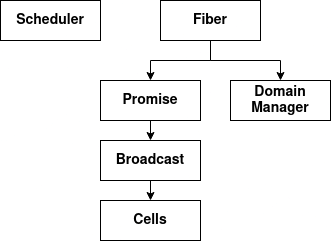
\includegraphics[width=0.75\textwidth]{Eio_Module_Hierarchy.png}
    \caption{Eio module hierarchy.}
    \label{fig:eio-module-hierarchy}
\end{figure}

Figure~\ref{fig:eio-module-hierarchy} shows the simplified module hierarchy of the concepts we focus on.
A standard arrow stands for a direct source code dependency from one module to another.
The diamond arrow between \ocamlin{Scheduler} and \ocamlin{Fiber} stands for the implicit dependency that fibers perform effects which are handled by code in the scheduler module.

Fibers can fork off new fibers using the \efork{} effect, suspend execution using the \esuspend{} effect, and get access to some context data using the \egetctx{} effect,
all of which are handled by the scheduler they are running in.
The implementation of the fiber and scheduler functions are discussed in section~\ref{sec:sched-impl}.
\emph{Promises} are built on top of the \emph{broadcast} data structure, which is a lock-free signalling construct that is used by fibers to signal other fibers when they are done.
The specification of promises is discussed in section~\ref{sec:sched-spec}.
Broadcast is based on the \emph{CQS} data structure, whose specification is already verified using Iris~\cite{koval2023cqs}, but Eio customizes the implementation so we had to adapt the proof.
We discuss this process in section~\ref{sec:broadcast}.
Fibers in Eio also have access to \emph{thread-local variables} by performing a \egetctx{} effect, which is discussed in section~\ref{sec:thread-local-vars}.
They are thread-local in the sense that they are shared between all fibers of one scheduler.
Finally, we discuss our addition of multithreading to the \hazel{} operational semantics in order to model running schedulers in different threads.
This turned out to be technically trivial, so we only discuss it in appendix~\ref{sec:apdx-mt} and take a multithreaded semantics and support for Iris \emph{shared invariants} as a given in the reminder of the main text.

\subsection{Contributions}
\label{sec:intro-contributions}

To summarize our contributions, in this thesis we verify the \textbf{safety} and \textbf{effect safety} of a simplified model of Eio which serves as an extended case study on the viability of \hazel{} for verifying programs with effect handlers.
This includes:

\begin{itemize}
    \item The verification of the basic Eio \textbf{fiber abstraction} running on a common denominator scheduler.
    \item Proving reusable specifications for the main three effects of Eio: \efork{}, \esuspend{}, and \egetctx{}.
    \item An adaptation of the existing verification of CQS to the customized version used by Eio.
    \item Adding multithreading to \hazel{}'s operational semantics, which shows we can reason about programs that use both \textbf{multithreading} and \textbf{effect handlers}.
\end{itemize}
